\subsection{Complejidad:}

Para analizar la complejidad voy a intentar representar cómo 'funciona' el algoritmo con una entrada de n trabajos.\\
La idea de esto es ver qué cosas calcula y de qué manera, para poder ver cuántas operaciones realiza en total.\\

Me pareció mejor esta forma en vez de un análisis linea por linea ya que se ve más detalladamente cómo actua el algoritmo. 
Además para no mezclar tantas cosas y que sea más legible voy a olvidarme de las partes de $agregar\_a\_maquina(j)$ (Líneas 4, 9 y 12 del pseudocódigo), esto obviamente no influye en la complejidad total ya que cada operación de ese tipo es O(1).\\

En principio se crea una matríz $n*n$ y se modifica la posición (0,1) con el costo del trabajo 1. Esto es O($n^{2}$) + O(1)= O($n^{2}$)\footnote{La matríz está implementada como vector de vectores}  (Líneas 2 y 3).\\

La posición (0,1) se calcula en O(1):\\

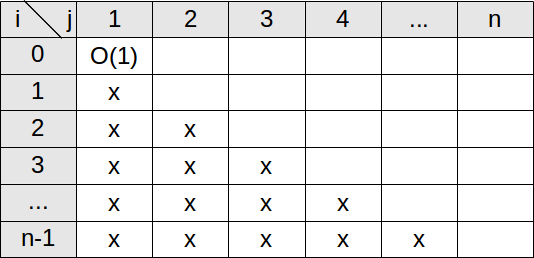
\includegraphics[scale=0.7]{ej1/complejidad1.png}\footnote{Los casilleros en blanco son los que faltan calcular y los que contienen una x nunca se calculan porque el For de la Línea 6 va desde i=0 hasta j-1.} \\

Luego, ingresamos en los For (Líneas 5 y 6). El algoritmo recorre las posiciones en blanco indicadas en el gráfico (la 'mitad' de la matriz si trazaramos una linea en diagonal) y para cada posición hace lo siguiente:\\

Si $i=j-1$ :\\
El algoritmo recorre las posiciones válidas de la columna anterior a la que se encuentra procesando, y busca el mínimo entre ellas (sumandole el costo de hacer j, Línea 8).\\
Por lo tanto se debe encontrar el mínimo de j-1 posiciones, esto es O(j-1).\\

Si $i\neq j-1$ :\\
La posición (i,j) de la matriz necesita sólo la posición (i,j-1) para ser calculada, esto es O(1) ya que se accede a la matriz y se suman enteros (Línea 11).\\

En resumen si $i=j-1$ es O(j-1) sino es O(1):\\

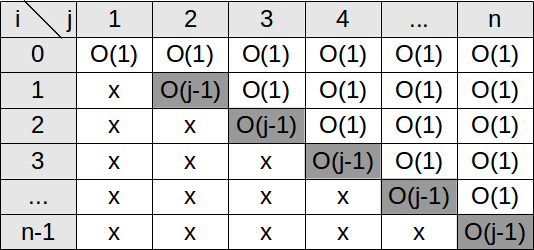
\includegraphics[scale=0.7]{ej1/complejidad2.png}\\

El algoritmo entonces recorre $ \sum_{j=2}^{n} (j-1)\ +\ n$ posiciones donde $ \sum_{j=2}^{n} (j-1)$ de ellas las resuelve en O(1) y el resto en O(j-1), que como j es a lo sumo n O(j-1)=O(n).\\

Puedo decir entonces que la complejidad final es hacer $\sum_{j=2}^{n} (j-1)$ veces $O(1)\ +\ n$ veces $O(n)$.\footnote{Disculpen el abuso de notación}\\

Ahora $\sum_{j=2}^{n} (j-1)\ =\ \frac{n^{2}-n}{2}$ por lo tanto es O($n^{2}$)\\

Complejidad del ciclo: $O(n^{2})\ *\ O(1)\ +\ O(n)\ *\ O(n)$ = $O(n^{2})\ *\ O(n^{2})$ = $O(2*n^{2})$ = $O(n^{2})$

La línea 16 es O(n) (recorre la última columna de la matriz).\\

\textbf{Entonces, complejidad total:}
$O(n^{2})\ +\ O(n^{2})\ +\ O(n)$ = $O(n^{2})$
